% Printable Holder Template for iPhone/iPad
% Manuel Parra 
% 

\documentclass[12pt,a4paper]{article}
\usepackage[utf8]{inputenc}
\usepackage[english]{babel}
\usepackage{amsmath}
\usepackage{amsfonts}
\usepackage{amssymb}
\usepackage{graphicx}
\usepackage{multicol}
\usepackage{tikz}
\usepackage{marvosym}
\usepackage{lmodern}
\usepackage[left=1.5cm,right=1.5cm,top=1cm,bottom=2cm]{geometry}

\author{Manuel Parra Royón }

\title{\textbf{Printable   iPhone/iPad  holder template in \LaTeX $ $ (incl. other mobiles and tablets)}}
\begin{document}

\maketitle
\thispagestyle{empty}

% Begin  
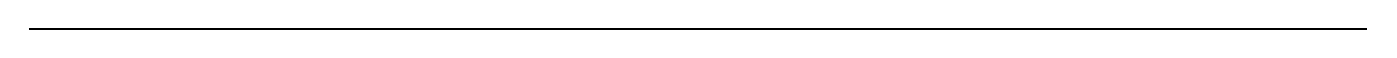
\begin{tikzpicture}
\draw[thick,rounded corners=3pt] (0,0) -- (17,0) ;  
\end{tikzpicture}


\begin{multicols}{2} 

% Plotting the figure with TIKZ (easy !)
 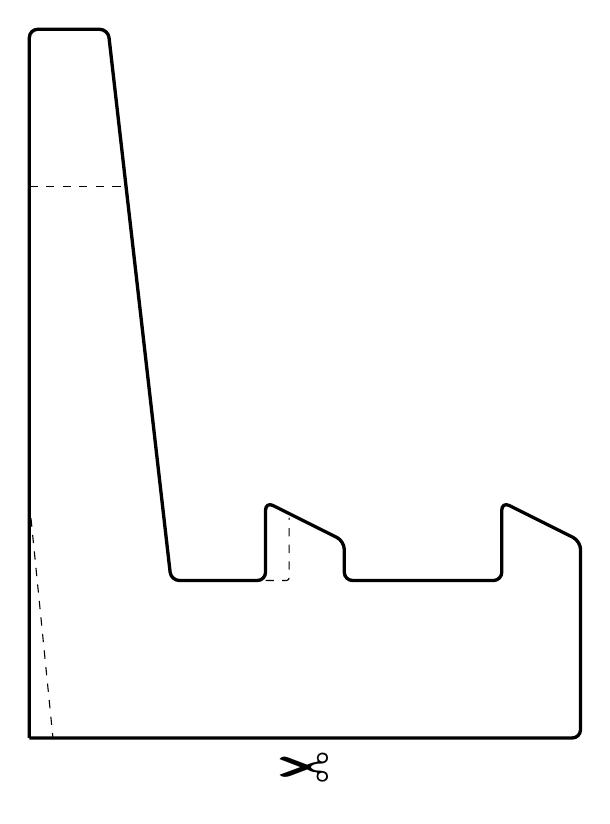
\begin{tikzpicture}
 % The figure
  \draw[very thick,rounded corners=3pt] (0,1) -- (0,10) -- (1,10)  -- (1.8,3) -- (3,3) -- (3,4) -- (4,3.5) -- (4,3) -- (6,3) -- (6,4) -- (7,3.5) -- (7,3)  -- ( 7,1 ) -- (0,1);  
  % Optional cuts with dashed lines
  \draw[dashed,rounded corners=1pt] (3,3) -- (3.3,3) -- (3.3,3.8);  
  \draw[dashed,rounded corners=1pt] (0,4) -- (0.3,1);  
  \draw[dashed,rounded corners=1pt] (0,8) -- (1.2,8);  
  % Plot scissors
  \node (scissors) at (3.5,0.6) {\Huge\Leftscissors};
 \end{tikzpicture}


% A few images of the process
\begin{center}
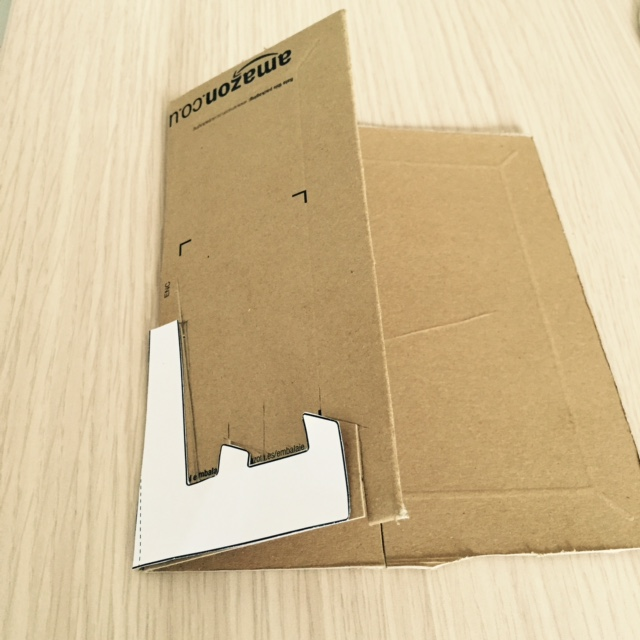
\includegraphics[scale=0.135]{img/holder_01}\\
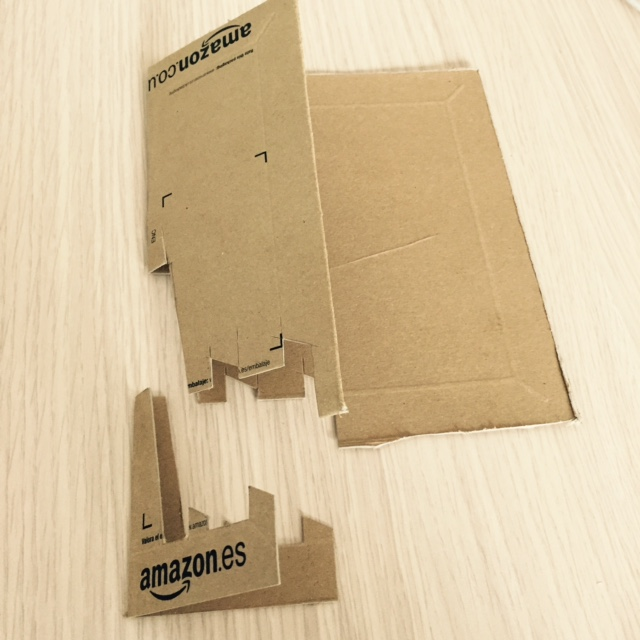
\includegraphics[scale=0.135]{img/holder_02}\\
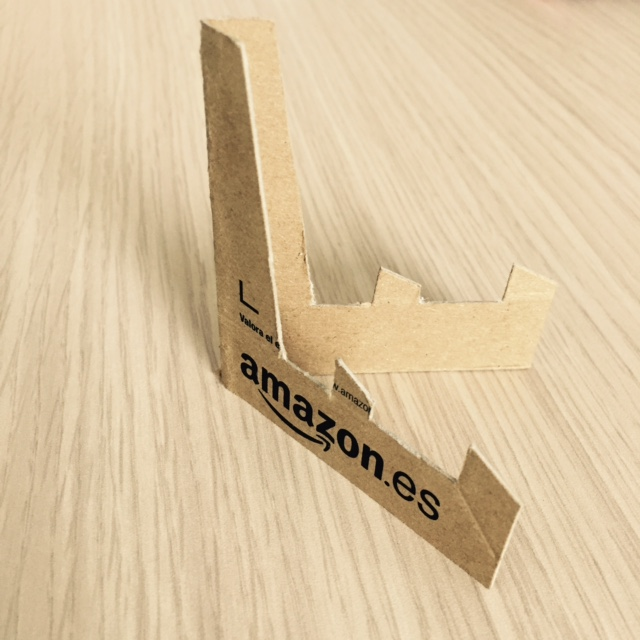
\includegraphics[scale=0.135]{img/holder_03}\\
\end{center}

\end{multicols}



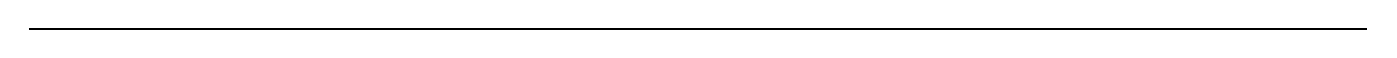
\begin{tikzpicture}
\draw[ thick,rounded corners=3pt] (0,0) -- (17,0) ;  
\end{tikzpicture}
% End 



\section*{Instructions}

\begin{multicols}{2}
\begin{enumerate}
\item Cut out the figure.
\item Take paper or something like cardboard and fold it in half. 
\item Place the cut out figure on the cardboard with the longest side against the fold, then trace the figure.
\item Cut out the figure traced on the carboard, leaving the fold uncut.
\item That's it!.
\end{enumerate}

\textit{Dashed lines are optional cuts }

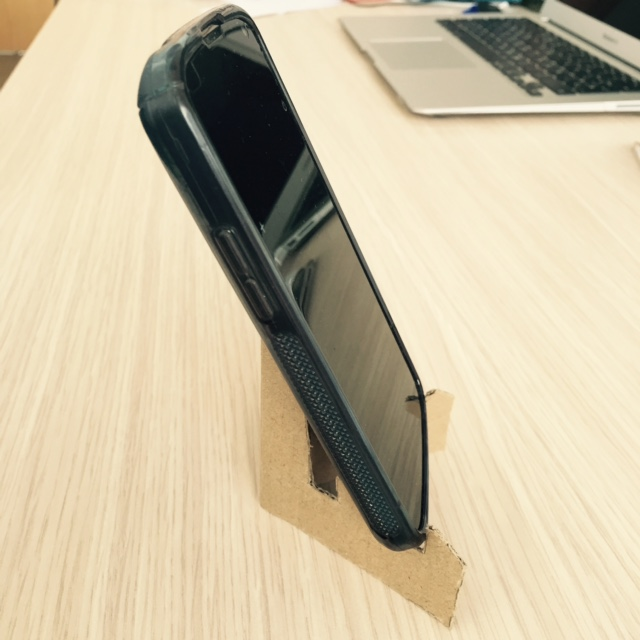
\includegraphics[scale=0.31]{img/holder_04}\\

\end{multicols}
  
\end{document}